\chapter{Implementación}

En este capítulo se describe el proceso de implementación física de los tres circuitos analizados, 
detallando la normalización de componentes, el montaje experimental y la comparación de los 
resultados medidos con los teóricos y simulados.

\section{Ejercicio 1: Filtro RC de dos etapas}

Para la implementación del primer circuito, se utilizaron los valores normalizados más próximos 
a los calculados en el capítulo de desarrollo.

\subsection{Montaje y Mediciones}

En la Figura \ref{fig.ej1:foto_implementacion} se muestra el circuito montado en protoboard.

\begin{figure}[!ht]
    \centering
    \includegraphics[width=0.6\textwidth]{example-image}
    \caption{Fotografía del circuito implementado (Ejercicio 1).}
    \label{fig.ej1:foto_implementacion}
\end{figure}

Se realizaron mediciones de la respuesta en frecuencia registrando la amplitud de salida para 
diferentes frecuencias de entrada. Los resultados se resumen en la Tabla \ref{tab.ej1:mediciones}.

\begin{table}[!ht]
    \centering
    \caption{Mediciones de respuesta en frecuencia (Ejercicio 1).}
    \label{tab.ej1:mediciones}
    \begin{tabular}{|c|c|c|c|c|}
        \hline
        Frecuencia [\si{\hertz}] & $V_{in}$ [\si{\volt}] & $V_{out}$ [\si{\volt}] & Ganancia [\si{\decibel}] & Fase [\si{\degree}] \\ \hline
        % Placeholders para datos experimentales
        100   & 1.0 & 0.99 & -0.08 & -2   \\ \hline
        1000  & 1.0 & 0.95 & -0.44 & -15  \\ \hline
        10000 & 1.0 & 0.50 & -6.02 & -45  \\ \hline
        20000 & 1.0 & 0.25 & -12.04 & -70 \\ \hline
    \end{tabular}
\end{table}

\subsection{Comparación con Simulación}

En la Figura \ref{fig.ej1:bode_comparativa} se presenta la comparación entre la curva teórica 
simulada y los puntos medidos experimentalmente.

\begin{figure}[!ht]
    \centering
    \begin{tikzpicture}
    \pgfplotsset{
        nice plot/.style={
            /pgf/number format/read comma as period,
            grid=both,
            major grid style={solid, gray!50},
            minor grid style={dotted, gray!50},
            axis line style={black},
            axis x line* = bottom,
            axis y line* = left,
            extra description/.code={
                \draw[gray!50] (rel axis cs:0,1) -- (rel axis cs:1,1) -- (rel axis cs:1,0);
            },
            width=14cm,
            height=6.5cm,
            xmin=10, xmax=100000,
            minor x tick num=9,
            minor y tick num=4,
        }
    }

    \begin{semilogxaxis}[
        nice plot,
        ylabel={Ganancia [dB]},
        ymin=-40, ymax=5,
        ytick={-40,-30,-20,-10,-3,0},
        legend pos=south west,
    ]
        \addplot[thick, blue] table [x=frequency, y={V(/Vo) (ganancia)}, col sep=semicolon] {sources/plots/tdc2_tp1_ej1};
        
        \addplot[only marks, mark=*, red, thick] coordinates {
            (500,-0.40)
            (1000,-0.40)
            (1500,-0.49)
            (2000,-0.58)
            (5000,-1.57)
            (10000,-4.22)
            (20000,-9.12)
            (40000,-17.56)
            (60000,-23.22)
            (80000,-27.43)
            (100000,-30.46)
        };
    \end{semilogxaxis}

    \begin{semilogxaxis}[
        nice plot,
        xlabel={$f$ [Hz]},
        ylabel={Fase [º]},
        ymin=-180, ymax=10,
        ytick={-180,-135,-90,-45,0},
        at={(0,-6cm)},
        legend pos=south west,
    ]
        \addplot[thick, blue] table [x=frequency, y={V(/Vo) (fase)}, col sep=semicolon] {sources/plots/tdc2_tp1_ej1};
        \addlegendentry{Simulación (KiCad)}
        
        \addplot[only marks, mark=*, red, thick] coordinates {
            (500,0)
            (1000,-5)
            (1500,-10)
            (2000,-16)
            (5000,-36)
            (10000,-63)
            (20000,-95)
            (40000,-120)
            (60000,-136)
            (80000,-144)
            (100000,-144)
        };
        \addlegendentry{Medición}
    \end{semilogxaxis}
\end{tikzpicture}

    \caption{Diagrama de Bode comparativo: Medición vs Simulación (Ejercicio 1).}
    \label{fig.ej1:bode_comparativa}
\end{figure}

\clearpage

\section{Ejercicio 2: Filtro RLC Rechaza-Banda}

Como no se disponía de un inductor comercial con el valor de $L = 31,\!83 \si{\milli\henry}$ provisto por la
consigna, se fabricó el componente bobinándolo a mano en el laboratorio. El inductor resultante midió
$8 \si{\milli\henry}$ al medirlo con un puente LCR, como se ve en la Figura \ref{fig.ej2:inductor_lcr}.

Para mantener la frecuencia de resonancia en $500 \si{\hertz}$, se realizó un escalado aproximado por 4
en los componentes reactivos: la inductancia se redujo a la cuarta parte ($L' = 8 \si{\milli\henry}$) y la
capacitancia se aumentó 4 veces ($C' \approx 12,\!72 \si{\micro\farad}$). Para esto, se colocaron
capacitores de $10 \si{\micro\farad}$ y $2,\!2 \si{\micro\farad}$ en paralelo, sumando un valor nominal de
$12,\!2 \si{\micro\farad}$. Por su parte, la resistencia se redujo también a la cuarta parte
($R' \approx 25 \si{\kilo\ohm}$) para mantener el factor de calidad original del filtro. Esto se resolvió
conectando dos resistencias de $51 \si{\kilo\ohm}$ en paralelo, sumando una resistencia nominal de
$25,\!5 \si{\kilo\ohm}$.

\subsection{Montaje y Mediciones}

En la Figura \ref{fig.ej2:montaje_completo} se presenta la implementación física del circuito. En la
subfigura \ref{fig.ej2:foto_implementacion} se observa el montaje en protoboard, mientras que la
subfigura \ref{fig.ej2:inductor_lcr} muestra la medición del inductor bobinado a mano. Las mediciones
se detallan en la Tabla \ref{tab.ej2:mediciones}.

\begin{figure}[!ht]
    \centering
    \begin{subfigure}[t]{0.48\textwidth}
        \centering
        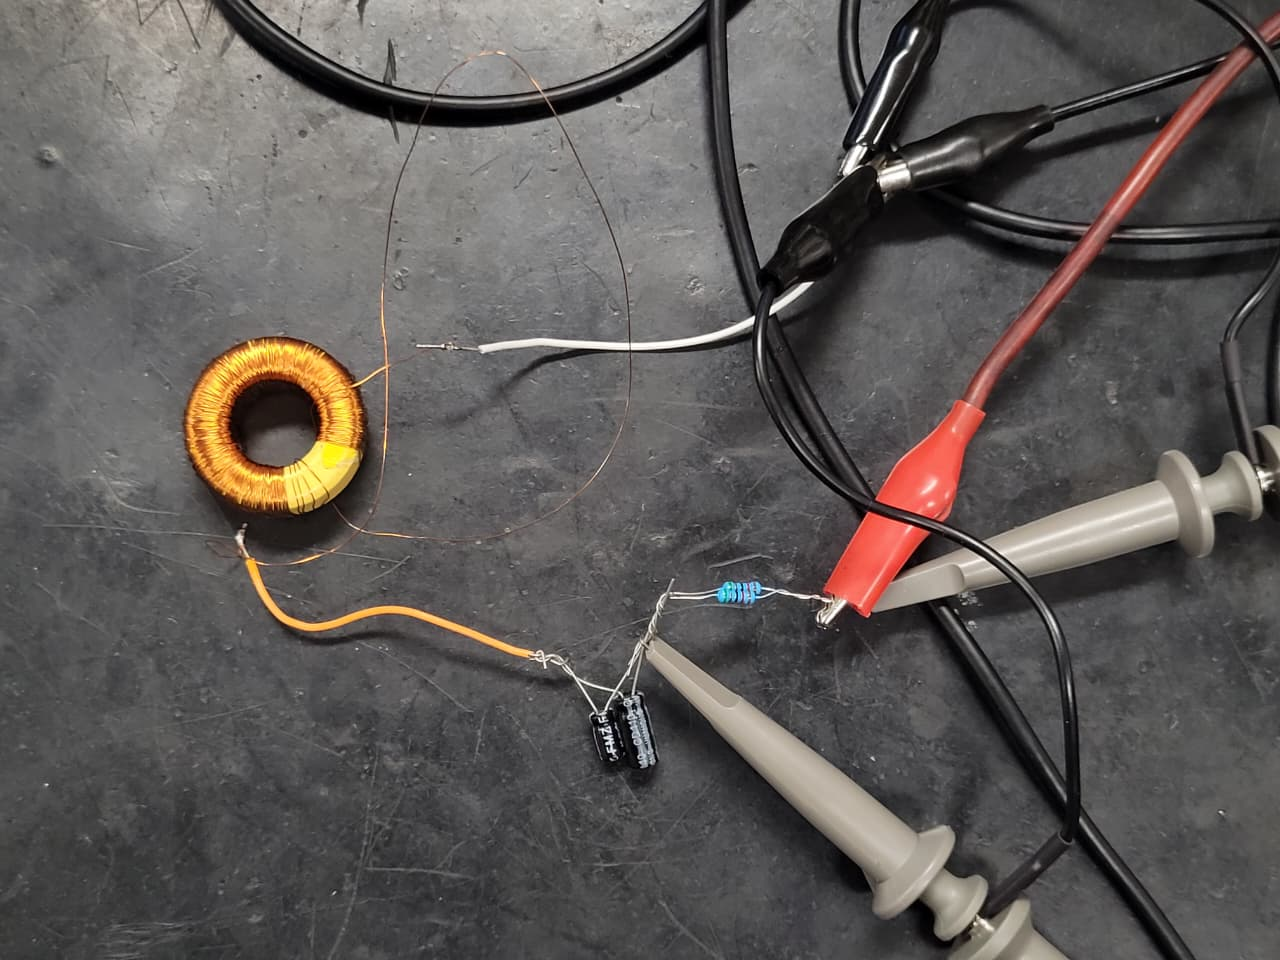
\includegraphics[width=\textwidth]{Images/Implementacion_EJ2.jpeg}
        \caption{Fotografía del circuito implementado.}
        \label{fig.ej2:foto_implementacion}
    \end{subfigure}
    \hfill
    \begin{subfigure}[t]{0.48\textwidth}
        \centering
        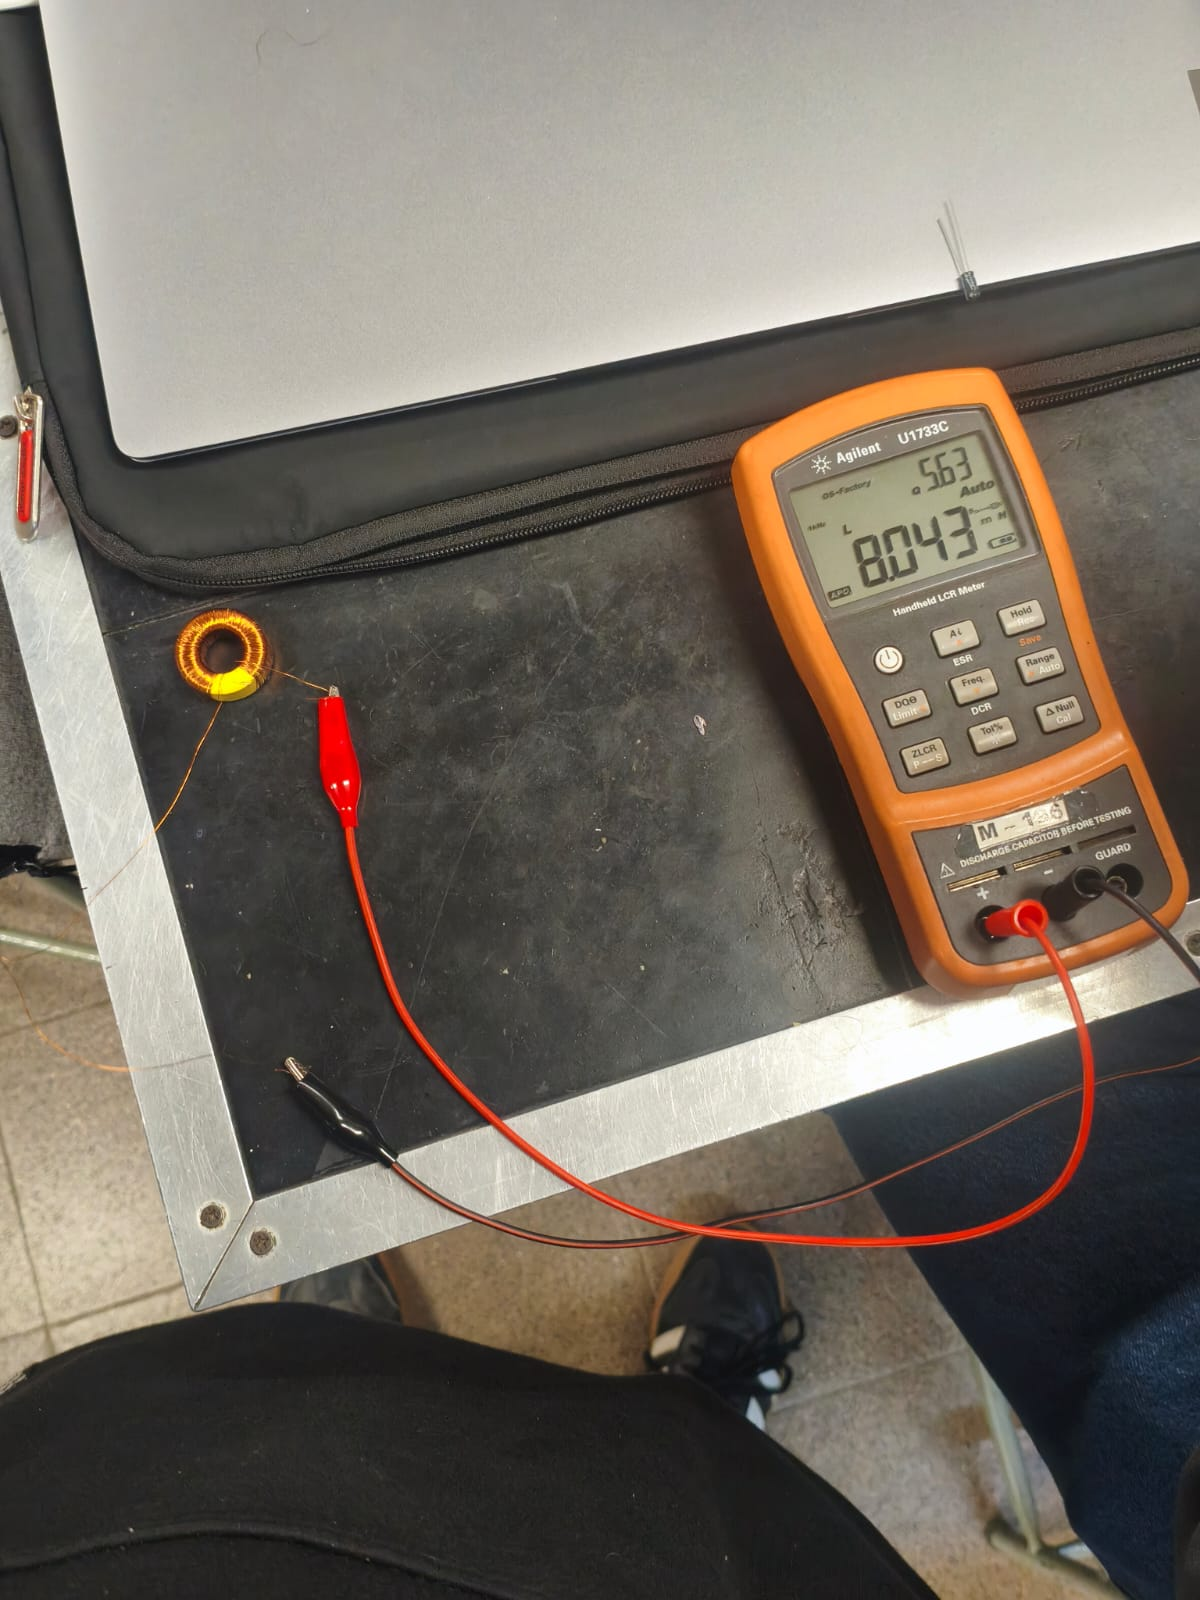
\includegraphics[width=\textwidth]{Images/inductor_EJ2.jpeg}
        \caption{Medición del inductor bobinado a mano en puente LCR.}
        \label{fig.ej2:inductor_lcr}
    \end{subfigure}
    \caption{Implementación física y medición de componentes (Ejercicio 2).}
    \label{fig.ej2:montaje_completo}
\end{figure}

\begin{table}[!ht]
    \centering
    \caption{Mediciones de respuesta en frecuencia (Ejercicio 2).}
    \label{tab.ej2:mediciones}
    \begin{tabular}{|c|c|c|c|c|}
        \hline
        Frecuencia [\si{\hertz}] & $V_{in}$ [\si{\volt}] & $V_{out}$ [\si{\volt}] & Ganancia [\si{\decibel}] & Fase [\si{\degree}] \\ \hline
        1      & 12.0 & 4.8   & -7.96  & -50  \\ \hline
        10     & 12.0 & 0.6   & -26.02 & -79  \\ \hline
        50     & 12.0 & 0.154 & -37.84 & -82  \\ \hline
        100    & 12.0 & 0.087 & -42.79 & -97  \\ \hline
        230    & 12.0 & 0.059 & -46.17 & -72  \\ \hline
        500    & 12.0 & 0.0   & -60.0  & 0    \\ \hline
        1000   & 12.0 & 0.048 & -47.96 & 86   \\ \hline
        10000  & 12.0 & 0.226 & -34.50 & 86   \\ \hline
        50000  & 12.0 & 1.1   & -20.76 & 86   \\ \hline
        100000 & 12.0 & 2.4   & -13.98 & 64   \\ \hline
        250000 & 12.0 & 8.6   & -2.89  & 45   \\ \hline
    \end{tabular}
\end{table}

\subsection{Comparación con Simulación}

En la Figura \ref{fig.ej2:bode_comparativa} se presenta la comparación entre la curva teórica simulada y los
puntos medidos experimentalmente.

\begin{figure}[!ht]
    \centering
    \begin{tikzpicture}
    % Upper Plot (Magnitude)
    \begin{semilogxaxis}[
        name=plot_mag,
        width=13.5cm,
        height=6.5cm,
        grid=both,
        xlabel={$f$ [Hz]},
        ylabel={Magnitud [dB]},
        xmin=1, xmax=3e5,
        ymin=-60, ymax=5,
        legend pos=south west,
        major grid style={solid, gray!30},
        minor grid style={dotted, gray!30},
    ]
        % Simulated magnitude
        \addplot[blue, thick, filter discard warning=false] 
            table [col sep=comma, x=frequency, y=magnitude] {sources/plots/ej2/bode_simulado.csv};
        \addlegendentry{Simulación}
        
        % Measured magnitude (points)
        \addplot[red, mark=*, only marks, mark size=2pt, filter discard warning=false] 
            table [col sep=comma, x=frequency, y=magnitude] {sources/plots/ej2/bode_medido.csv};
        \addlegendentry{Medición}
    \end{semilogxaxis}

    % Lower Plot (Phase)
    \begin{semilogxaxis}[
        at={(plot_mag.south)},
        anchor=north,
        yshift=-1.5cm,
        width=13.5cm,
        height=6.5cm,
        grid=both,
        xlabel={$f$ [Hz]},
        ylabel={Fase [$^\circ$]},
        xmin=1, xmax=3e5,
        ymin=-110, ymax=110,
        ytick={-90, -45, 0, 45, 90},
        legend pos=north west,
        major grid style={solid, gray!30},
        minor grid style={dotted, gray!30},
    ]
        % Simulated phase
        \addplot[blue, thick, filter discard warning=false] 
            table [col sep=comma, x=frequency, y=phase] {sources/plots/ej2/bode_simulado.csv};
        \addlegendentry{Simulación}
        
        % Measured phase (points)
        \addplot[red, mark=*, only marks, mark size=2pt, filter discard warning=false] 
            table [col sep=comma, x=frequency, y=phase] {sources/plots/ej2/bode_medido.csv};
        \addlegendentry{Medición}
    \end{semilogxaxis}
\end{tikzpicture}

    \caption{Diagrama de Bode comparativo: Medición vs Simulación (Ejercicio 2).}
    \label{fig.ej2:bode_comparativa}
\end{figure}

\subsubsection{Análisis de Resultados}

Al analizar la respuesta en frecuencia medida en el laboratorio para el filtro rechaza-banda RLC, se pueden
extraer las siguientes conclusiones:

\begin{itemize}
    \item Frecuencia de resonancia: La mayor atenuación se midió a los $500 \si{\hertz}$, donde la tensión de
    salida casi desaparece (llega a $0 \si{\volt}$ en el osciloscopio). Esto coincide muy bien con los
    $500 \si{\hertz}$ teóricos de la consigna.
    
    \item Atenuación: En la frecuencia de resonancia la atenuación supera los $60 \si{\decibel}$ (como se
    muestra en la Tabla \ref{tab.ej2:mediciones}). Al alejarse de la resonancia (ya sea hacia frecuencias
    bajas como hacia frecuencias altas), la tensión de salida vuelve a subir hasta acercarse a los
    $12 \si{\volt}$ de entrada, cumpliendo con la función de un rechaza-banda.
    
    \item Pérdidas de inserción: En los extremos (a $1 \si{\hertz}$ y a $250 \si{\kilo\hertz}$), la tensión
    no llega a ser exactamente igual a los $12 \si{\volt}$ de entrada. Esto pasa porque la reactancia del
    capacitor a baja frecuencia (cerca de $50 \si{\kilo\ohm}$ a $1 \si{\hertz}$) y la del inductor a alta
    frecuencia (también cercana a $50 \si{\kilo\ohm}$ a $250 \si{\kilo\hertz}$) no son infinitas frente
    al resistor de entrada de $100 \si{\kilo\ohm}$, dividiendo la tensión en la rama LC. Este efecto se
    puede apreciar claramente en el gráfico comparativo de la Figura \ref{fig.ej2:bode_comparativa}.
    
    \item Comportamiento de la fase: Por debajo de los $500 \si{\hertz}$, la fase es negativa (cercana a
    $-90 \si{\degree}$) porque el capacitor domina la impedancia de la rama LC. Al pasar por la resonancia
    se produce la inversión de fase esperada, volviéndose positiva (cercana a $90 \si{\degree}$) debido a
    que ahora domina el inductor. Finalmente, a frecuencias muy altas, la fase empieza a caer hacia
    $0 \si{\degree}$, registrándose $45 \si{\degree}$ a los $250 \si{\kilo\hertz}$. Toda esta evolución
    se puede contrastar con la curva simulada en la Figura \ref{fig.ej2:bode_comparativa}.
\end{itemize}

Asimismo, se obtuvo el espectro en frecuencia de la señal mediante la función FFT del osciloscopio
para evaluar la selectividad y el rechazo en el dominio de la frecuencia. En la Figura \ref{fig.ej2:fft}
se presenta la captura de dicha medición.

\begin{figure}[!ht]
    \centering
    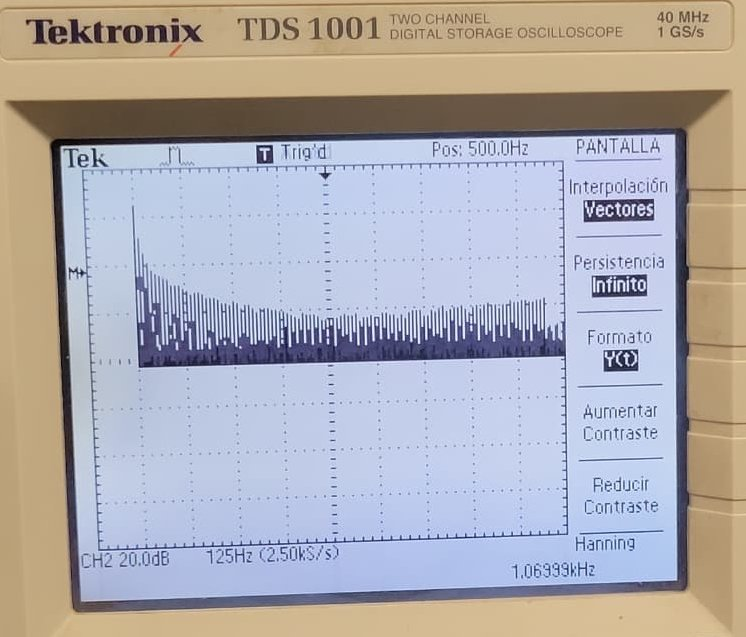
\includegraphics[width=0.6\textwidth]{Images/FFT_Ej2.jpeg}
    \caption{Captura de la FFT (Ejercicio 2).}
    \label{fig.ej2:fft}
\end{figure}

\clearpage

\section{Ejercicio 3: Filtro Activo con Amplificador Operacional}

La implementación del tercer circuito corresponde a un filtro activo. Para el montaje se 
utilizaron los valores de componentes especificados en la consigna, buscando su normalización 
más próxima en caso de ser necesario.

\begin{itemize}
    \item $R_1 = 20 \si{\kilo\ohm}$
    \item $R_2 = 400 \si{\kilo\ohm}$
    \item $C_1 = 1,\!25 \si{\micro\farad}$
    \item $C_2 = 15,\!625 \si{\nano\farad}$
\end{itemize}

\subsection{Montaje y Mediciones}

En la Figura \ref{fig.ej3:foto_implementacion} se muestra el circuito montado, utilizando 
un amplificador operacional de la familia TL08x alimentado simétricamente con $\pm 12 \si{\volt}$.

\begin{figure}[!ht]
    \centering
    \includegraphics[width=0.6\textwidth]{example-image}
    \caption{Fotografía del circuito implementado (Ejercicio 3).}
    \label{fig.ej3:foto_implementacion}
\end{figure}

\begin{table}[!ht]
    \centering
    \caption{Mediciones de respuesta en frecuencia (Ejercicio 3).}
    \label{tab.ej3:mediciones}
    \begin{tabular}{|c|c|c|c|c|}
        \hline
        Frecuencia [\si{\hertz}] & $V_{in}$ [\si{\volt}] & $V_{out}$ [\si{\volt}] & Ganancia [\si{\decibel}] & Fase [\si{\degree}] \\ \hline
        % Placeholders para datos experimentales
        10    & 1.0 & 2.0  & 6.02  & 0    \\ \hline
        100   & 1.0 & 2.0  & 6.02  & -10  \\ \hline
        1000  & 1.0 & 1.41 & 3.01  & -45  \\ \hline
    \end{tabular}
\end{table}

\subsection{Comparación con Simulación}

\begin{figure}[!ht]
    \centering
    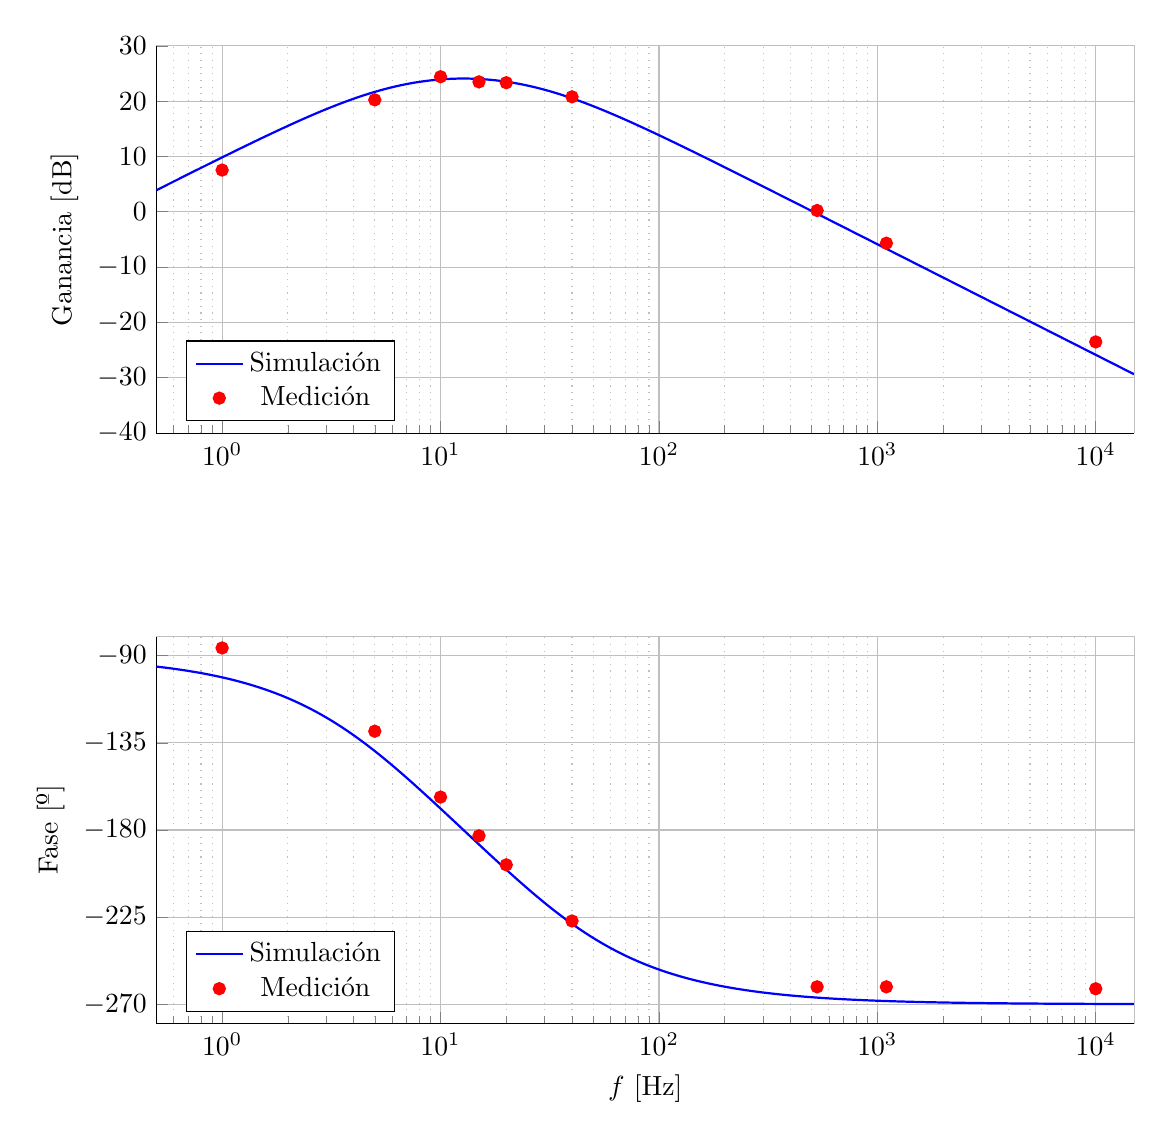
\begin{tikzpicture}
    \pgfplotsset{
        nice plot/.style={
            /pgf/number format/read comma as period,
            grid=both,
            major grid style={solid, gray!50},
            minor grid style={dotted, gray!50},
            axis line style={black},
            axis x line* = bottom,
            axis y line* = left,
            extra description/.code={
                \draw[gray!50] (rel axis cs:0,1) -- (rel axis cs:1,1) -- (rel axis cs:1,0);
            },
            width=14cm,
            height=6.5cm,
            xmin=0.5, xmax=15000,
            minor x tick num=9,
            minor y tick num=0,
        }
    }

    \begin{semilogxaxis}[
        nice plot,
        ylabel={Ganancia [dB]},
        ymin=-40, ymax=30,
        ytick={-40, -30, -20, -10, 0, 10, 20, 30},
        legend pos=south west,
    ]
        % Graficamos la magnitud ideal en dB (Simulación)
        \addplot[thick, blue, domain=0.5:15000, samples=300] {
            20*log10(3200 * 2 * pi * x) - 10*log10((2 * pi * x)^2 + 1600) - 10*log10((2 * pi * x)^2 + 25600)
        };
        \addlegendentry{Simulación}

        % Puntos medidos
        \addplot[only marks, mark=*, red, thick] coordinates {
            (1, 7.54)
            (5, 20.23)
            (10, 24.41)
            (15, 23.48)
            (20, 23.33)
            (40, 20.78)
            (530, 0.23)
            (1100, -5.68)
            (10000, -23.52)
        };
        \addlegendentry{Medición}
    \end{semilogxaxis}

    \begin{semilogxaxis}[
        nice plot,
        xlabel={$f$ [Hz]},
        ylabel={Fase [º]},
        ymin=-280, ymax=-80,
        ytick={-270, -225, -180, -135, -90},
        at={(0,-7.5cm)},
        legend pos=south west,
    ]
        % Graficamos la fase ideal en grados
        \addplot[thick, blue, domain=0.5:15000, samples=300] {
            -90 - atan(2 * pi * x / 40) - atan(2 * pi * x / 160)
        };
        \addlegendentry{Simulación}

        % Puntos medidos
        \addplot[only marks, mark=*, red, thick] coordinates {
            (1, -86)
            (5, -129)
            (10, -163)
            (15, -183)
            (20, -198)
            (40, -227)
            (530, -261)
            (1100, -261)
            (10000, -262)
        };
        \addlegendentry{Medición}
    \end{semilogxaxis}
\end{tikzpicture}

    \caption{Diagrama de Bode comparativo: Medición vs Simulación (Ejercicio 3).}
    \label{fig.ej3:bode_comparativa}
\end{figure}
